\section{Concept Generation and
Evaluation}\label{concept-generation-and-evaluation}

Creativity is a great motivator because it makes people interested in
what they are doing. Crea­tivity gives hope that there can be a
worthwhile idea. Creativity gives the possibility of some sort of
achievement to everyone. Creativity makes life more fun and more
interesting.---Edward DeBono

When developing a design, it is important to explore many potential
solutions and select the best one from them. Too often a single concept
is generated and is the only one pursued, the unfortunate result being
that potentially better solutions are not considered. When confronted
with a problem, engineers must explore different concepts, critically
evaluate them, and be able to defend the decisions that led to a
particular solution. Two key thought processes employed are creativity
and judgment. Creativity involves the generation of novel con­cepts,
while judgment is applied to evaluate and select the best solution for
the problem. Creativity and judgment appear to be inherent individual
qualities that can't be taught. That is to some extent true, but with
practice and application of formal techniques, they can be im­proved.

It is important to distinguish between innovation and creativity.
Creativity refers to the ability to develop new ideas, while innovation
is the ability to bring creative ideas to reality. Innovation is valued
by companies since new products and services are often their life­blood.
That is why many make it a priority to hire engineers who can bring
creativity to the design process. This chapter addresses creativity,
concept generation, and evaluation in design. The first part describes
barriers to creative thought, followed by strategies for overcoming them
and enhancing creativity. Next, methods for concept generation are
presented, followed by techniques for concept evaluation.

Learning Objectives

By the end of this chapter, the reader should:

\begin{itemize}
\item
  Understand the importance of creativity, innovation, concept
  generation, and concept evaluation in engineering design.
\item
  Be familiar with the barriers that hinder creativity.
\item
  Be able to apply strategies and formal methods for concept generation.
\item
  Be able to apply techniques for the evaluation of design concepts.
\end{itemize}

\subsection{Creativity}\label{creativity}

Is creativity something that is inherent in the individual or something
that can be learned? It appears that both are true; some individuals are
naturally more creative than others, yet people can enhance their
creativity with conscious effort and practice. This section examines
barriers to creativity, different thinking modes, and strategies for
enhancing creativity. One of the ways to spark creativity is to solve
puzzles. To get into the creative spirit the reader can try to solve the
puzzles presented in Figure 4.1.

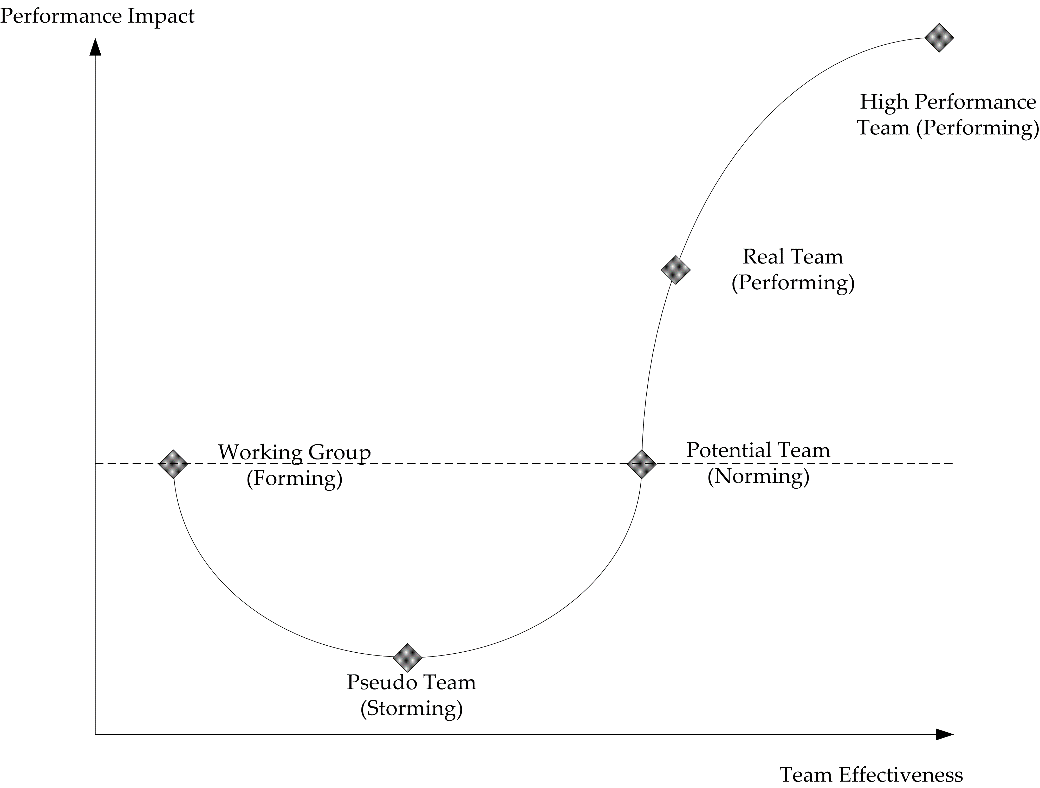
\includegraphics[width=0.66667in,height=1.30208in]{media/image1.emf}
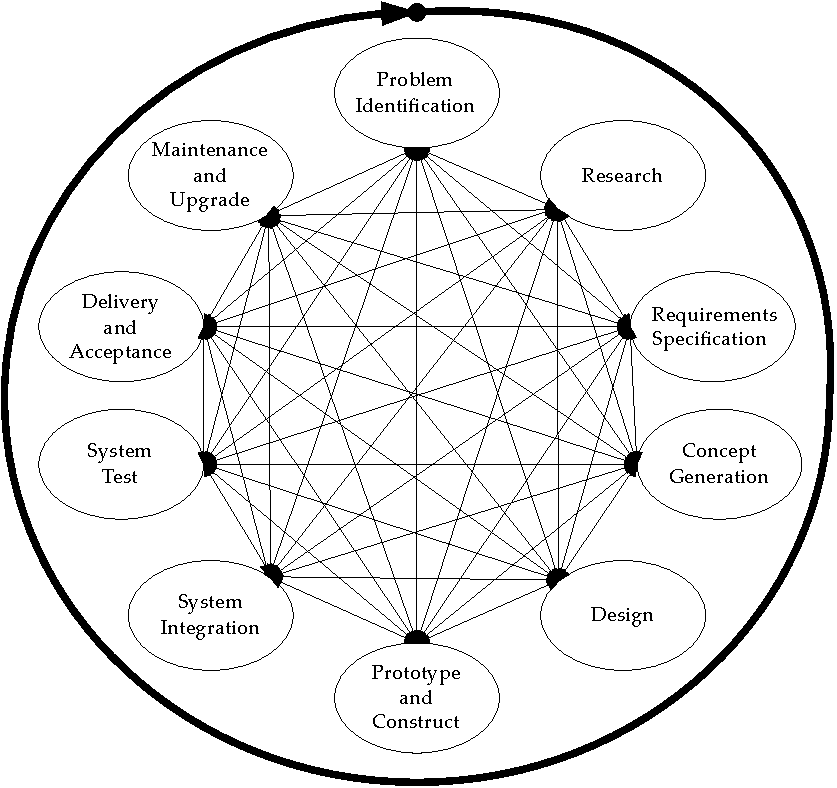
\includegraphics[width=1.30208in,height=1.30208in]{media/image2.emf}

(a) (b)

\textbf{Figure 4.1} (a) The shovel problem. Think of this as a shovel
with a coin on the spade. The ob­jective is to move two lines so that the
coin is no longer in the spade, but there is still a shovel. (b) The
nine dot problem. Draw four connected straight lines that pass through
all nine dots.

\subsubsection{Barriers to Creativity}\label{barriers-to-creativity}

James L. Adams, an engineer and former professor at Stanford University,
has researched in­novation in technical domains. He examined the barriers
to creativity and classified them into the following four types: 1)
perceptual blocks, 2) emotional blocks, 3) cultural and environ­mental
blocks, and 4) intellectual and expressive blocks {[}Ada01{]}.

\emph{Perceptual blocks} are those that prevent people from clearly
seeing the problem for what it is. A common perceptual block is the
tendency to delimit the problem space, or in other words, to put
constraints on the problem that don't exist. Have you solved the puzzles
shown in Figure 4.1 yet? If not, it is possible that you are placing
constraints on the problems that don't exist. Knowing that this is the
case, you may want to go back and try again. Another example of a
perceptual block is the tendency to stereotype or see a solution to a
problem that one is biased to see. This occurs because we have used
similar techniques for solving the problem in the past. For example, if
you have used a microcontroller to solve a certain type of problem,
chances are that you are going to consider using a microcontroller in
all related problems in the future. Another perceptual block is the
difficulty of isolating the true problem. Three pictures that illustrate
this are shown in Figure 4.2. When examining these images, people tend
to form a conclusion as to what the content of each one is. Look
carefully, as each picture has two equally valid interpretations.

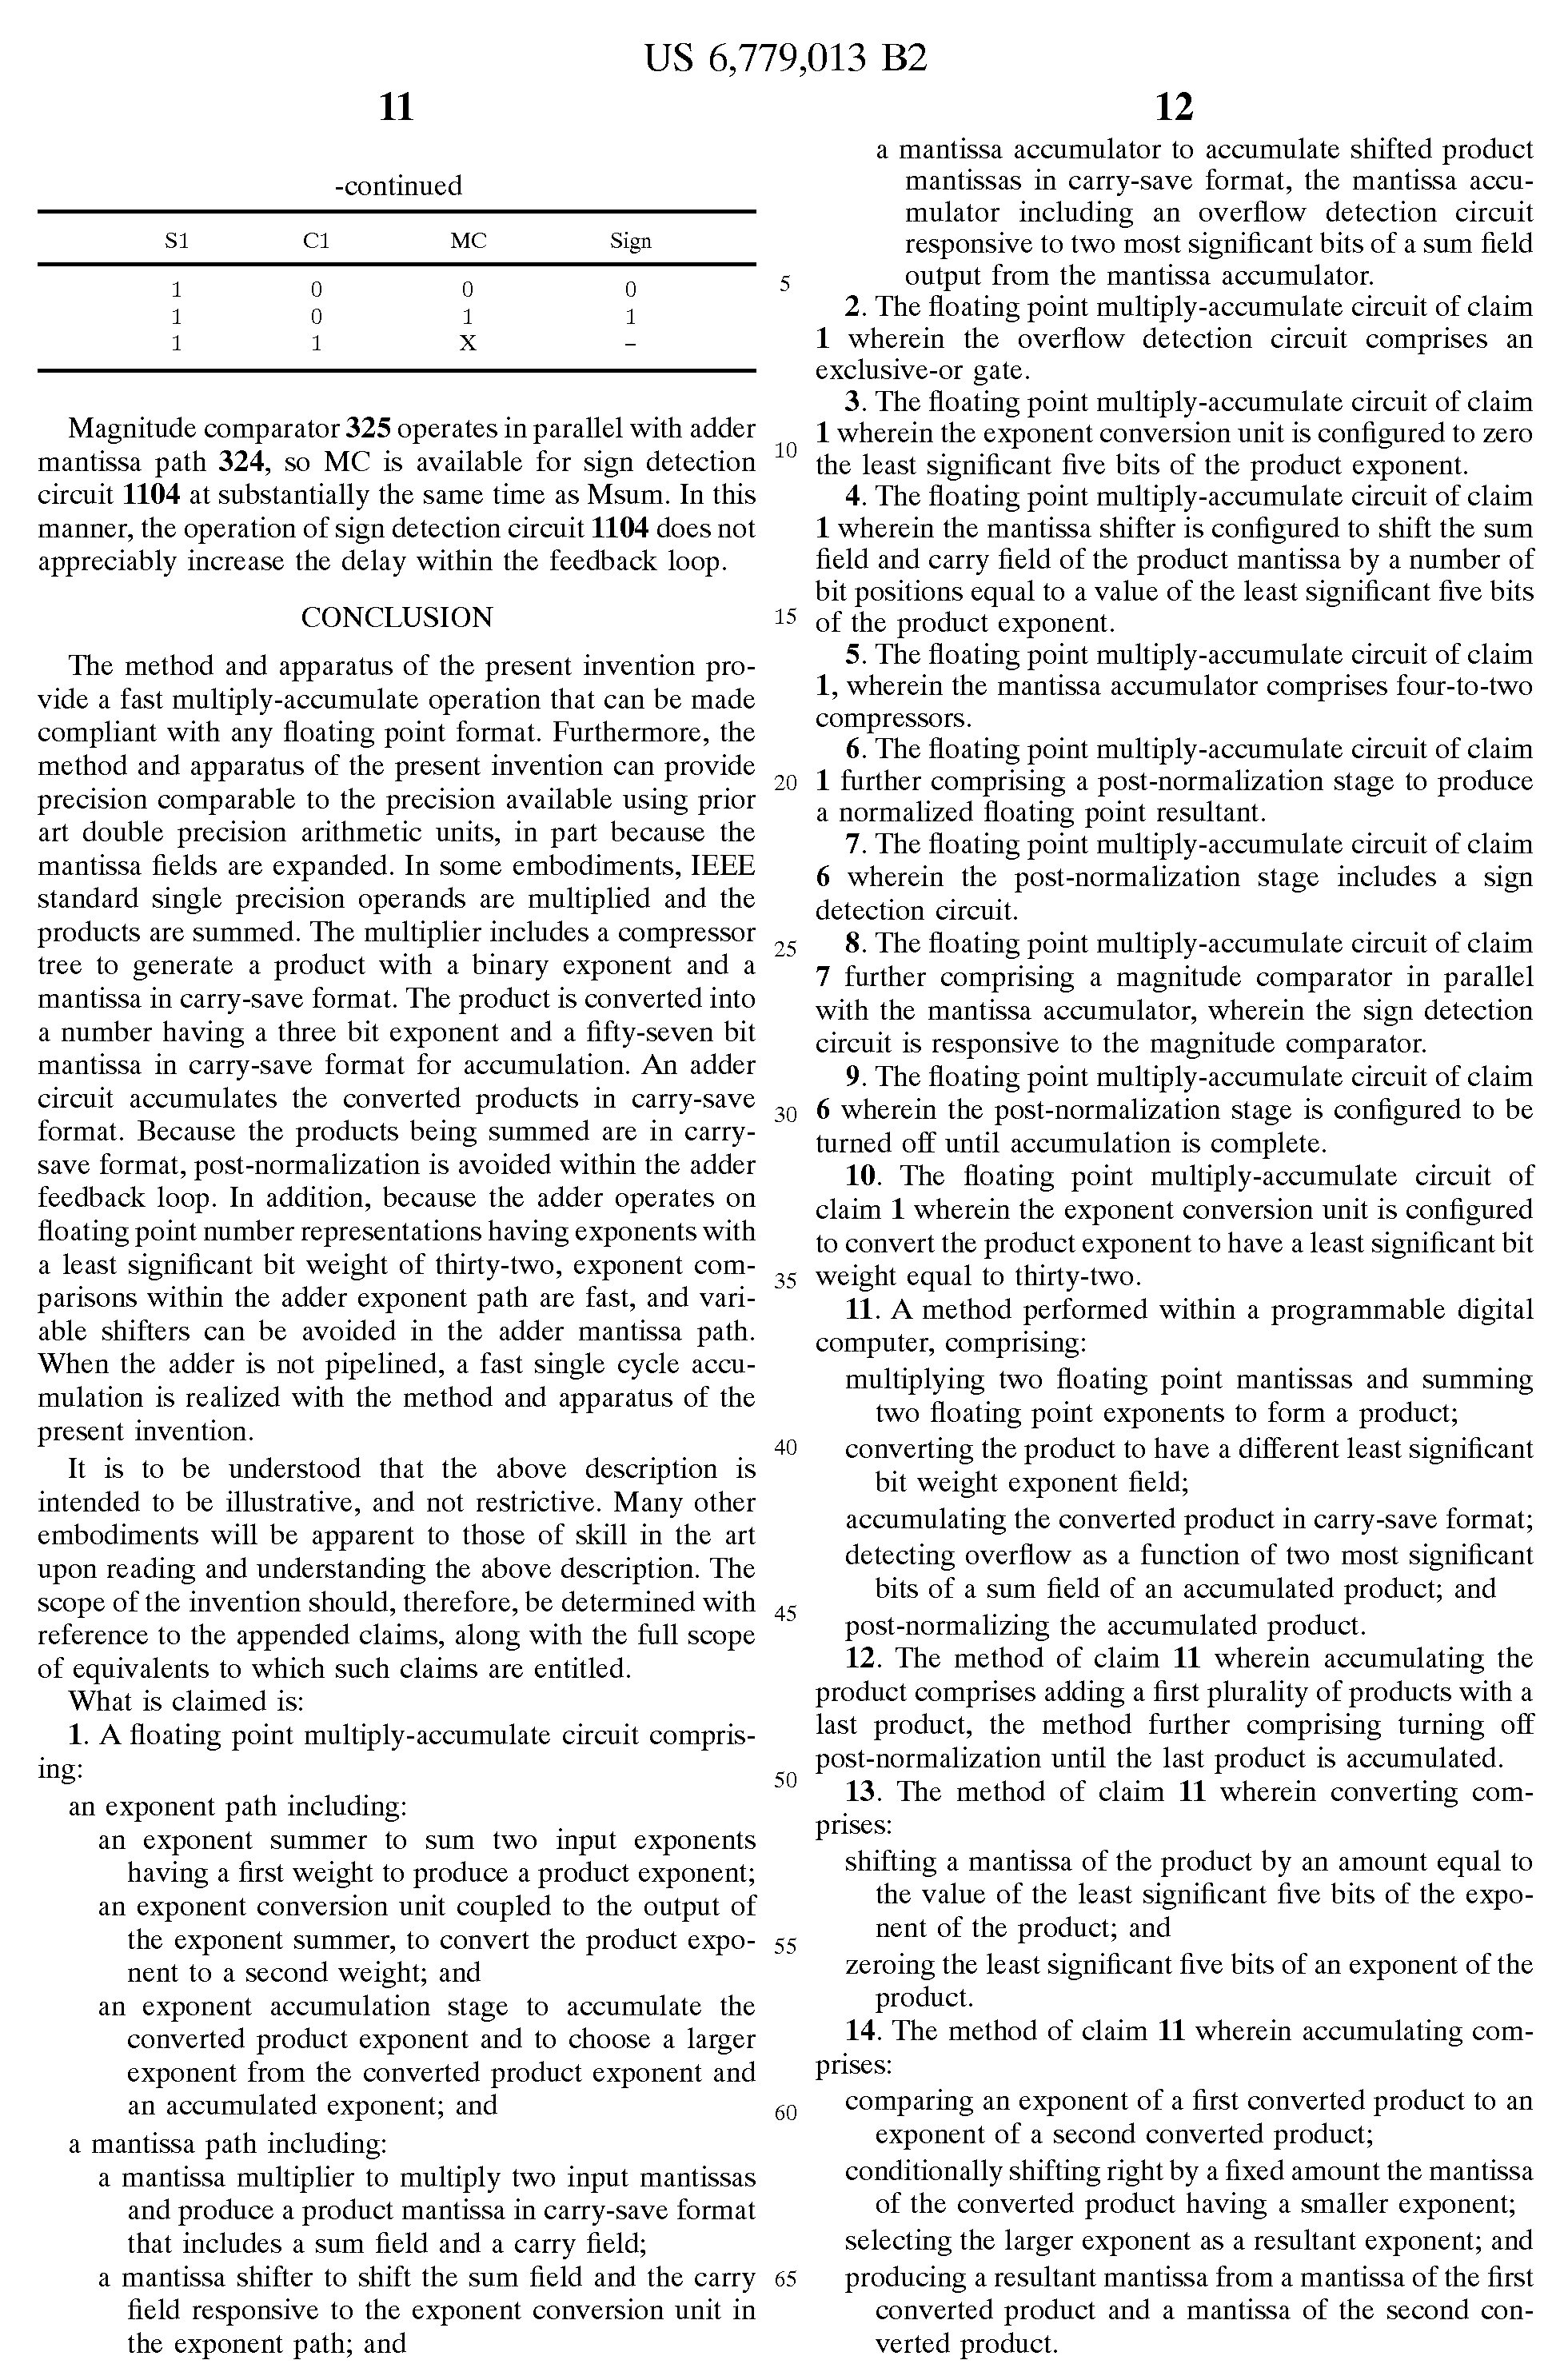
\includegraphics[width=1.58333in,height=2.20833in]{media/image3.png}
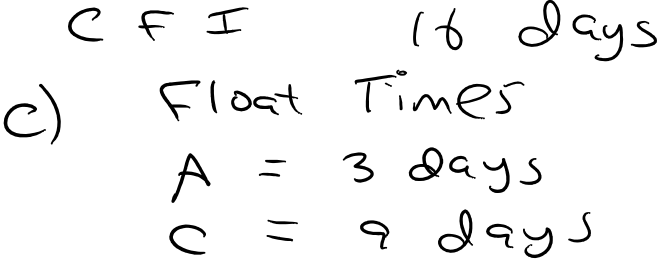
\includegraphics[width=1.59375in,height=2.19792in]{media/image4.png}

\includegraphics[width=1.89583in,height=2.19792in]{media/image5.png}

\textbf{Figure 4.2} Each of the images shown above has two different
interpretations. Can you determine what they are?

One of the most common \emph{emotional blocks} is the fear of failure.
People often have creative ideas, but are afraid to express them since
they may be criticized or may not have the ``correct'' answer. It is
cliché to hear that you must fail often to succeed, but true. The highly
successful product design company, IDEO, that was examined in Chapter 2
takes the approach in con­cept generation to ``\emph{fail early and
often}'' in order to succeed {[}Kel01{]}. Their design teams are
en­couraged to develop many seemingly outlandish ideas that are often
discarded, but some­times lead to innovative solutions. Another emotional
block is a fear of chaos and disorgani­zation. The creative process
challenges engineers, since it is disorganized and not a neat scien­tific
approach to which they are accustomed. Another block is the tendency to
critically judge ideas, rather than generate and build upon them.
Finally, it takes time for creative ideas to incubate. Most of us can
relate to the experience when we could not solve a problem that nagged
us for a period of time, followed by that unexpected \emph{``Aha!''}
moment when we identi­fied the solution.

\emph{Environmental blocks} refer to those things in our environment
that limit creative ability. This could be in the form of poor teamwork
where members distrust each other and criticize each other's ideas. In
the workplace, this could be due to autocratic management that resists
new ideas. There are also cultural biases against creativity. There is a
bias against creativity as an approach to problem solving in the
engineering field. This is usually based upon the reasoning that there
is a single correct solution to a problem and creativity is an excuse
for poor engineering. It is true that creativity and brainstorming alone
do not solve engineering problems---the concepts generated need to be
scrutinized using engineering principles to become viable innovations.

The final block that Adams identified is that of \emph{intellectual and
expressive}. In an engi­neering context, this means that the designer
needs to have an understanding of intellectual tools that are applied to
solve problems. For example, mathematics is a universal language for
expressing and solving scientific problems. Specific examples in ECE are
languages that de­scribe the characteristics of systems such as
functional, logical, and state behaviors. Examples in digital design are
truth tables (input, output behavior) and state diagrams
(stimulus-response). In the domain of electronics design, a functional
approach (input, output, and function) is commonly used. Chapters 5 and
6 present tools for modeling the behavior of ECE systems.

\subsubsection{Vertical and Lateral
Thinking}\label{vertical-and-lateral-thinking}

Edward DeBono is the father of a field known as \emph{\textbf{lateral
thinking}}, which offers a different per­spective on the barriers to
creativity. Lateral thinking is contrasted to what is known as the
vertical thinking process {[}Deb67, Deb70{]}. Engineers tend to be
vertical (or convergent) think­ers, meaning that they are good at taking
a problem and proceeding logically to the solution. This is typically a
sequential linear process, where the engineer starts at the highest
level and successively refines elements of the design to solve the
problem. This is usually based upon experience solving similar problems
and conventional tools that are employed in that par­ticular area.

The objective of lateral (or divergent) thinking is to identify creative
solutions. It is not concerned with developing the solution for the
problem, or right or wrong solutions. It encourages jumping around
be­tween ideas. In the words of DeBono ``\emph{The vertical thinker says:
\textquotesingle I know what I am looking for.\textquotesingle{} The
lateral thinker says: \textquotesingle I am looking but I
won\textquotesingle t know what I am looking for until I have found
it.\textquotesingle{}} '' The field of lateral thinking is characterized
by puzzles of the following type found at Paul Sloane's Lateral Thinking
Puzzles website {[}\url{http://dspace.dial.pipex.com/sloane}{]}:

\begin{quote}
A body is discovered in a park in Chicago in the middle of summer. It
has a fractured skull and many other broken bones, but the cause of
death was hypothermia.

A hunter aimed his gun carefully and fired. Seconds later, he realized
his mistake. Minutes later, he was dead.

A man is returning from Switzerland by train. If he had been in a
non-smoking car he would have died.
\end{quote}

The objective in these puzzles is to develop plausible scenarios that
explain how each of the above situations could have happened. A solution
for the first example is that a person stowed away in the wheel
compartment of a jet airliner. While in flight he froze and died of
hypo­thermia. When the plane prepared to land, it lowered its landing
gear, causing the body to fall to the park, fracturing his skull, and
breaking his bones. Can you develop plausible scenarios that describe
each of them?

Vertical thinking focuses on sequential steps toward a solution and
tries to determine the correctness of the solution throughout the
process. This is very different from lateral thinking where there is
nonlinear jumping around between steps and there is no attempt to
discern be­tween right and wrong. As such, lateral thinking is more apt
to follow least likely paths to a solution, whereas vertical thinking
follows the most likely paths. The goal in lateral thinking is to
develop as many solutions as possible, while vertical thinking tries to
narrow to a single solution.

Lateral thinking is appropriate for the concept generation phase. So
should concept gen­eration and brainstorming be done by the individual or
by a team? DeBono and Osborn {[}Osb63{]} conclude that creativity is
more effective by individuals than by teams. However, Osborn also points
out that there is great value in applying creativity in teams, since it
provides a place for the team to work together on problems and see other
perspectives. Our anecdotal observations of student design teams
supports this---group brainstorming is effective for developing
concepts, new product ideas, new features, and different ways to combine
technologies. This is because in groups, ideas are readily built upon by
other team members. More mathe­matical, technical, and theoretical
breakthroughs tend to be the work of the lone genius. Ex­amples of this
are the Theory of Relativity (Einstein), Boolean Logic (Bool), and
Shannon's Sampling Theorem. We have also observed that novice designers,
who do not have much experience in concept generation, can benefit
greatly from group brainstorming techniques.

\subsubsection{Strategies to Enhance
Creativity}\label{strategies-to-enhance-creativity}

There are valuable strategies that can be employed to enhance the
creative process. The body of research on the subject is very large and
key points are summarized as follows:

\begin{itemize}
\item
  \emph{Have a questioning attitude.} One of the keys is to have a
  questioning attitude and chal­lenge assumptions. The willingness to do
  this generally decreases as people age. Young children are highly
  creative and are constantly questioning everything, with questions
  such as ``\emph{Why do trees have leaves?}'' or ``\emph{Why is the sky
  blue?}'' Asking basic questions stimulates creativity and is
  applicable to technical designs. When examin­ing a design with a
  microcontroller, ask questions such as ``\emph{Is there a way to
  replace the microcontroller?}''\emph{,} ``\emph{Are there other
  features that I can achieve with the microcontroller?}''\emph{,} and
  ``\emph{Is there a better microcontroller that can be used?}''
\item
  \emph{Practice being creative.} Research shows that people can improve
  their creative ability through conscious effort. For example, try
  solving the puzzles presented in this chapter and in the end of the
  chapter problems. Be conscious of things that bother you (``pet
  peeves'') in your everyday life and try to develop new solutions for
  them.
\item
  \emph{Suspend judgment.} It is easy to criticize and immediately
  dismiss ideas, so it is impor­tant to defer judgment and be flexible in
  thinking. Seemingly outlandish ideas can lead to other concepts that
  are valuable solutions. The opportunity for new solutions is curtailed
  if ideas are immediately judged and discarded. Creative concepts can
  be developed by taking a concept and modifying it or combining it with
  other seemingly unrelated concepts.
\item
  \emph{Allow time.} The creative process needs time for incubation. The
  human mind needs time to work on problems, so set aside time to
  reflect on the problem and to allow it to incubate so that the
  ``\emph{Aha!}'' moment of discovery can happen.
\item
  \emph{Think like a beginner.} New solutions often come from novices.
  The reason is that nov­ices don't have preconceived ideas as to the
  solution for a problem. Experience is a double-edged sword---it allows
  one to quickly solve problems by drawing upon pre-existing solutions,
  but can inhibit creativity. If confronted with a new problem that
  bears similarity to one encountered in the past, then it is likely
  that the new solution will bear similarity to the old one. If everyone
  else is it doing it one way, consider the opposite.
\end{itemize}

Many creative ideas arise from novel combinations and adaptations of
existing technology. SCAMPER, an acronym for Substitute, Combine, Adapt,
Modify, Put to other use, Eliminate, and Rearrange/Reverse, can be used
as a guide to systematically generate creative concepts. The SCAMPER
principles are valuable in brainstorming and are described below:

\begin{itemize}
\item
  \emph{Substitute.} Can new elements be substituted for those that
  already exist in the system?
\item
  \emph{Combine.} Can existing entities be combined in a novel way that
  has not been done be­fore?
\item
  \emph{Adapt.} Can parts of the whole be adapted to operate
  differently?
\item
  \emph{Modify.} Can part or all of a system be modified? For example,
  size, shape, or functional­ity.
\item
  \emph{Put to other use.} Are there other application domains where the
  product or system can be put to use?
\item
  \emph{Eliminate.} Can parts of the whole be eliminated? Or should the
  whole itself be elimi­nated?
\item
  \emph{Rearrange or Reverse.} Can elements of the system be rearranged
  differently to work bet­ter? This is different from substituting in
  that the elements of the system are not changed, but rearranged or
  ordered differently to create something new. In terms of reversal, are
  there any roles or objectives that can be reversed?
\end{itemize}

SCAMPER is a modification of a set of questions that was originally
posed by Osborn {[}Osb63{]} and was modified to its form above by
Michalko {[}Mic91{]}.

\subsection{Concept Generation}\label{concept-generation}

After the problem is defined, the next step is to explore concepts for
the solution. It is unlikely that a design team will have reached this
stage without some ideas for solving the problem, but it is important to
fully explore the design space. Ullrich and Eppinger {[}Ull03{]}
identify the following phases of concept generation -- search
internally, search externally, and systematically explore. Each is
considered in turn.

External searching was covered to a great extent in Chapters 2 and 3,
which addressed conducting background research and benchmarking. Methods
of external searching are:

\begin{itemize}
\item
  Conduct literature search.
\item
  Search and review existing patents.
\item
  Benchmark similar products.
\item
  Interview experts.
\end{itemize}

Internal searching is done by the team members via methods such as
brainstorming. The team members need have to have a common problem
definition for this to be effective. Understanding the tradeoffs using
requirement analysis methods in Chapter 3 is also valuable, as
overcoming tradeoffs leads to innovative solutions. Furthermore, the
team should decompose larger problems into sub-problems and the attack
the sub-problems individually. Chapter 5 addresses the process of
problem decomposition.

\textbf{DILBERT\textsuperscript{®} by Scott Adams}


\includegraphics[width=5.48958in,height=1.95833in]{media/image6.png}

\subsubsection*{Figure 4.3 Wally brainstorming. (Dilbert © United
Feature Syndicate. Reprinted by
permission.)}\label{figure-4.3-wally-brainstorming.-dilbert-united-feature-syndicate.-reprinted-by-permission.}
\addcontentsline{toc}{subsubsection}{Figure 4.3 Wally brainstorming.
(Dilbert © United Feature Syndicate. Reprinted by permission.)}

The most well-known method of internal searching is
\emph{\textbf{brainstorming}}. Group brainstorming is effective for
generating many concepts in a short period of time. Experienced design
teams are known to generate hundreds of concepts in an hour. Traditional
brainstorming is not highly-structured---though a facilitator
helps---and employs five basic rules:

\begin{itemize}
\item
  No criticism or judgment of ideas.
\item
  Wild ideas are encouraged.
\item
  Quantity is stressed over quality.
\item
  Build upon and modify the ideas of others.
\item
  All ideas are recorded.
\end{itemize}

Many novice design teams struggle with unstructured brainstorming and
more formalized approaches, such as brainwriting and the Nominal Group
Technique, can be of benefit. The steps of \emph{\textbf{brainwriting}}
are:

\begin{enumerate}
\def\labelenumi{\arabic{enumi}.}
\item
  The team develops a common problem statement that is read out loud.
\item
  Each team member writes their ideas down on a card and places it in
  the center of the table.
\item
  Other team members then take cards from the pile and use other's ideas
  to generate new ones or build upon them, keeping in mind the
  principles of SCAMPER. Alternatively, members can each generate an
  idea, write it on a card, and then pass it to another team member.
  Each member then builds upon the idea passed to them.
\end{enumerate}

\emph{\textbf{Brainwriting 6-3-5}} is a variation where the objective is
to have six people, develop three ideas in five minutes. The optimal
number of people for the exercise is thought to be six, although it is
not necessary. Each person generates three ideas in five minutes, and
clearly describes it using sketches and written descriptions on paper.
At the end of five minutes, each team member passes their ideas to
another team member. The next person reviews the ideas of their teammate
and adds three more by building on them, developing new ones, or
ignoring as necessary. This process continues until all members have
reviewed all papers.

In the \emph{\textbf{Nominal Group Technique}} (NGT) {[}Del71{]} each
team member silently generates ideas that are reported out in a
round-robin fashion so that all members have an opportunity to present
their ideas. Concepts are selected by a multi-voting scheme with each
member casting a predetermined number of votes for the ideas presented.
The ideas are then ranked, discussed further, and voted upon again if
necessary. The steps of NGT are as follows:

\begin{itemize}
\item
  \emph{Read problem statement.} It should be read out loud by a team
  member (the facilitator).
\item
  \emph{Restate the problem.} Each person restates the problem in their
  own words to ensure that all members understand it.
\item
  \emph{Silently generate ideas}. All members silently generate ideas
  during a set period of time, typically 5--15 minutes.
\item
  \emph{Collect ideas in a round-robin fashion}. Each person presents
  one idea in turn until all ideas are exhausted. The facilitator should
  clarify ideas and all should be written where the entire team can view
  them.
\item
  \emph{Summarize and rephrase ideas.} Once the ideas are collected, the
  facilitator leads a discus­sion to clarify and rephrase the ideas. This
  ensures that the entire group is familiar with them. Related ideas can
  be grouped or merged together.
\item
  \emph{Vote.} Each person casts a predetermined number of votes,
  typically three to six, for the ideas presented. The outcome is a set
  of prioritized ideas that the team can further discuss and pursue.
\end{itemize}

To systematically generate concepts, the problem is decomposed
sub-functions and solutions are sought for the sub-functions. A
\emph{\textbf{concept table}}, demonstrated in Table 4.1, is a tool for
identifying different combinations, arrangements, and substitutions. The
table headings identify functions to be achieved in the design, while
the entries in the corresponding column represent po­tential solutions.
Novel products or solutions are generated by combining elements from
each of the columns, which are identified in the table by circled
elements. The solutions can be in the form of a single element selected
from each column, or as in the example shown, multiple elements selected
from each column.

\textbf{Table 4.1} A concept table for generating ideas for a personal
computing system. The potential so­lution is identified by the
combination of circled elements.

\begin{longtable}[]{@{}
  >{\raggedright\arraybackslash}p{(\columnwidth - 8\tabcolsep) * \real{0.2036}}
  >{\raggedright\arraybackslash}p{(\columnwidth - 8\tabcolsep) * \real{0.1965}}
  >{\raggedright\arraybackslash}p{(\columnwidth - 8\tabcolsep) * \real{0.2039}}
  >{\raggedright\arraybackslash}p{(\columnwidth - 8\tabcolsep) * \real{0.1970}}
  >{\raggedright\arraybackslash}p{(\columnwidth - 8\tabcolsep) * \real{0.1990}}@{}}
\toprule\noalign{}
\begin{minipage}[b]{\linewidth}\raggedright
\textbf{User Interface}
\end{minipage} & \begin{minipage}[b]{\linewidth}\raggedright
\textbf{Display}
\end{minipage} & \begin{minipage}[b]{\linewidth}\raggedright
\textbf{Connectivity \& Expansion}
\end{minipage} & \begin{minipage}[b]{\linewidth}\raggedright
\textbf{Power}
\end{minipage} & \begin{minipage}[b]{\linewidth}\raggedright
\textbf{Size}
\end{minipage} \\
\midrule\noalign{}
\endhead
\bottomrule\noalign{}
\endlastfoot
Keyboard & CRT & Serial \&

Parallel & Battery & Hand-held, Fits in pocket \\
Touchpad & Flat Panel & USB & AC Power & Notebook size \\
Handwriting Recognition & Plasma & Wireless Ethernet & Solar Power &
Wearable \\
Video & Heads-up Display & Wired Ethernet & Fuel Cell & Credit Card
Size \\
Voice & LCD & PCMCIA & Thermal Transfer & Flexible in shape \\
& & Modem /

Telephone & & \\
\end{longtable}

Based on the concepts circled in Table 4.1, one can imagine a personal
computing system that has the following features: 1) is wearable with
different credit card size components placed on the body and in clothing
to make it comfortable to use; 2) is powered by a combina­tion of solar
cells, fuel-cells, and from thermal heat generated by a person's body;
3) has a mi­crophone and camera integrated in the user's clothing for
interface to the system, as well as a flexible foldable keyboard for
typing that is stored in a pocket; 4) has a heads-up display inte­grated
with the user's eyeglasses or baseball hat; and 5) has a miniature
earpiece microphone used for communication. While the above example
focused on novel combinations and substitu­tions, the concept table can
also be used to examine the possibility of eliminating ideas. For
example, the table inherently assumes that a display will be used.
However, it should also be asked if it is abso­lutely necessary in the
design.

Another example is shown in Table 4.2, where the objective is to
identify design concepts for a temperature measurement and display
device. There are three main elements to the pro­posed solution: the
thermal sensing method, circuitry that converts the sensor in­formation
(temperature) to a voltage, and a display unit that converts the voltage
to a dis­played temperature. Note that the table implies a three-stage
architecture, thus concepts are generated within that framework. There
may be completely different architec­tures that are better.

\textbf{Table 4.2} Concept table for a temperature measurement device.

\begin{longtable}[]{@{}
  >{\raggedright\arraybackslash}p{(\columnwidth - 4\tabcolsep) * \real{0.3361}}
  >{\raggedright\arraybackslash}p{(\columnwidth - 4\tabcolsep) * \real{0.3319}}
  >{\raggedright\arraybackslash}p{(\columnwidth - 4\tabcolsep) * \real{0.3319}}@{}}
\toprule\noalign{}
\begin{minipage}[b]{\linewidth}\raggedright
\textbf{Thermal Sensing}
\end{minipage} & \begin{minipage}[b]{\linewidth}\raggedright
\textbf{Conversion to Voltage}
\end{minipage} & \begin{minipage}[b]{\linewidth}\raggedright
\textbf{Display}
\end{minipage} \\
\midrule\noalign{}
\endhead
\bottomrule\noalign{}
\endlastfoot
Thermistor & Op Amp Design & Seven-Segment LEDs \\
RTD & Transistor Designs & LCD \\
Thermocouple & & Analog Dial Indicator \\
\end{longtable}

A related tool is a \emph{\textbf{concept fan,}} which is a graphical
representation of design decisions and choices. An example concept fan
for the temperature measuring device is shown in Figure 4.4. Design
decisions are identified by circles; solutions are indicated by squares.
In this example, more options are shown than in Table 4.2. Concepts are
generated by selecting among the different solution blocks.

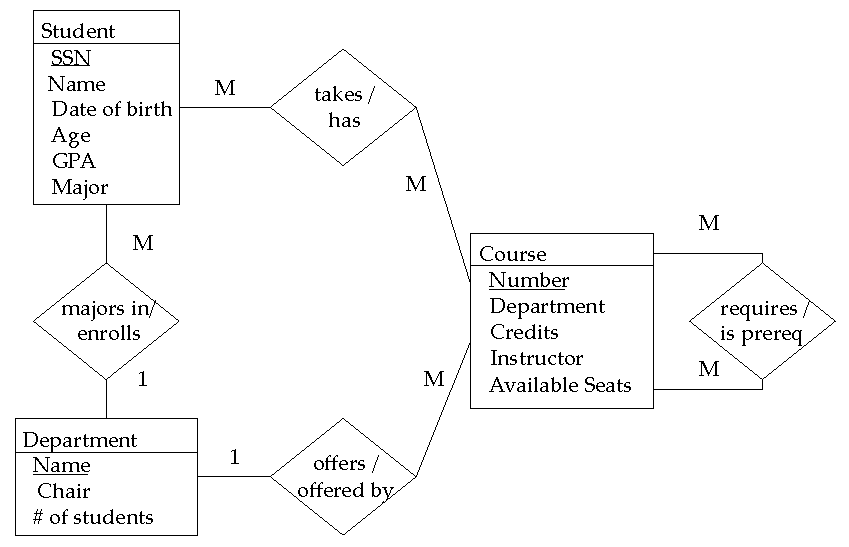
\includegraphics[width=5.47917in,height=3.19792in]{media/image7.emf}

\textbf{Figure 4.4} A concept fan for the temperature measuring device.
The circles represent the choices to be made and the squares represent
potential solutions to the choices.

\subsection{Concept Evaluation}\label{concept-evaluation}

The concepts generated are evaluated to determine which are the most
promising to pursue. The designer should exercise engineering judgment
and use the customer needs and technical factors to drive the decision.
This process is shown in Figure 4.5, where the user needs, concepts, and
engineering consideration serve as inputs to a decision process to ranks
the concepts. A point of caution---some of the methods presented
generate numerical scores for comparing concepts, leading one to
potentially believe that the quantita­tive results are infallible. Keep
in mind that the inputs are based on qualitative and semi-quantitative
assessments and can be geared to select a preconceived notion of the
solution. It is important to maintain flexibility of thinking, to
challenge assumptions, and ultimately determine the best concept.

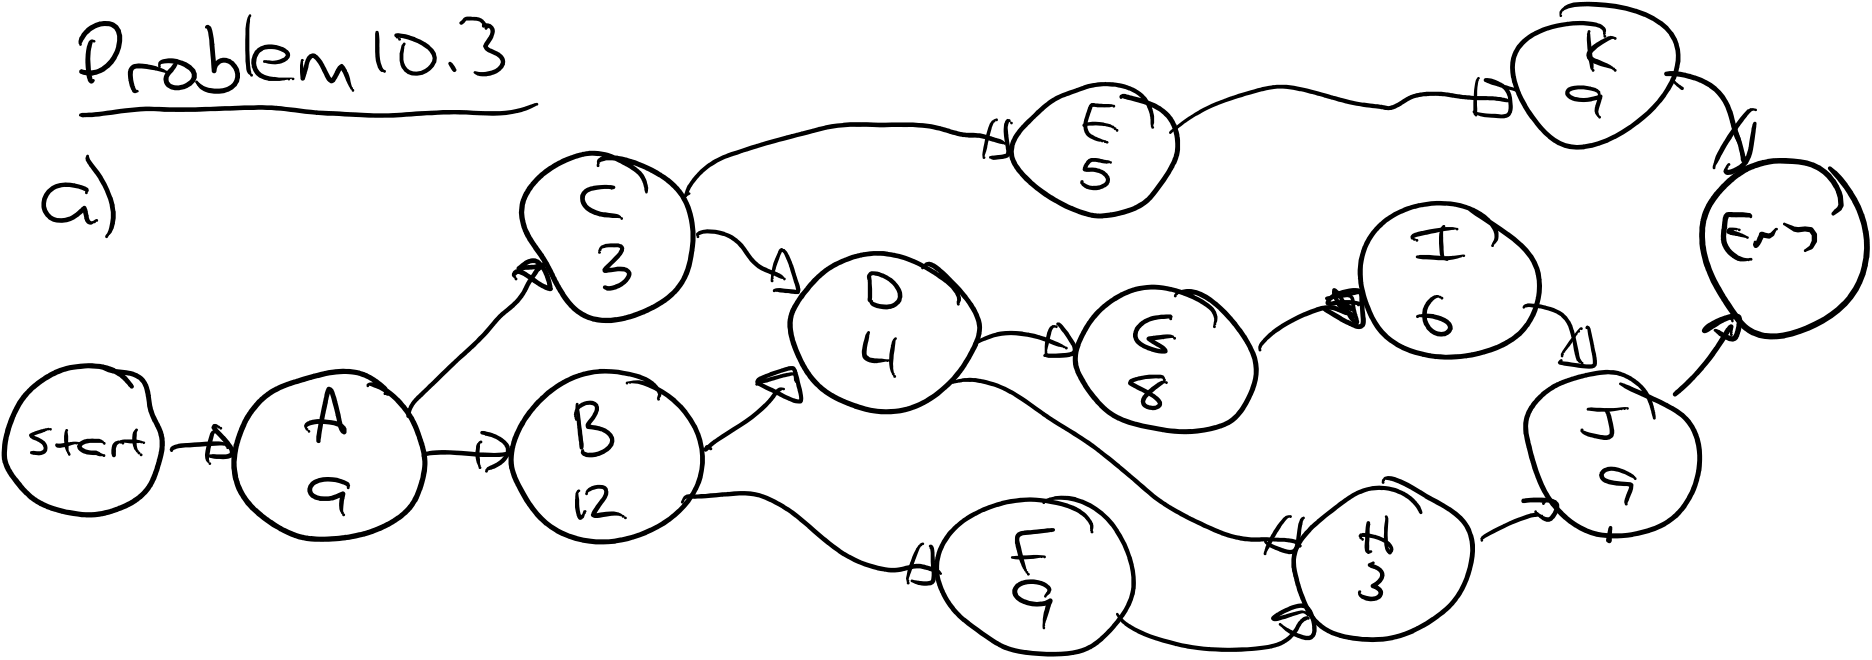
\includegraphics[width=3.35417in,height=1.3125in]{media/image8.emf}

\textbf{Figure 4.5} Process for concept evaluation.

\subsubsection{Initial Evaluation}\label{initial-evaluation}

The concepts generated should be initially reviewed and those that are
completely infeasible discarded. Some of the reasons a concept may be
deemed infeasible are that it may be far too costly, will take too long
to develop, or involve too much risk. In many cases it may be deemed
that using cutting-edge technology represents an unacceptable risk.
Concepts that clearly cannot meet the engineering requirements should
also be discarded. Care should be taken not to completely eliminate
ideas that may have merit, as conditions change and some concepts that
were previously thought unrealistic may become viable in the future.

\subsubsection{Strengths and Weaknesses
Analysis}\label{strengths-and-weaknesses-analysis}

Another form of evaluation is to complete a \emph{\textbf{strengths and
weaknesses analysis}} of the potential solutions. Table 4.3 demonstrates
the application of this analysis applied to an experi­mental design
project for testing of the Intel 1000XF card (examined in Chapter 2
(Example 2.2) and Chapter 3 (Table 3.2)). In order to test the card
under different operating temperatures, a method of heating the card and
holding its temperature fixed during the experiment was needed. The two
solutions compared were to use a contact heating element or to place the
card in an environmental test chamber. In this particular example, the
temperature chamber solution was ultimately selected due to the need for
a uniform temperature distribution. The strength and weakness analysis
is good for examining problems of moderate complexity. It suffers in
that it does not require uniform criteria for comparison. To make the
method more quantitative, relative scores for the strengths (plus
factors) and weaknesses (minus factors) can be assigned and used to
score the concepts.

\textbf{Table 4.3} A strengths and weaknesses analysis of proposed
methods for heating an Intel 1000XF card to be used in lifetime testing.
{[}Ese03{]}.

\begin{longtable}[]{@{}
  >{\raggedright\arraybackslash}p{(\columnwidth - 4\tabcolsep) * \real{0.2636}}
  >{\raggedright\arraybackslash}p{(\columnwidth - 4\tabcolsep) * \real{0.3636}}
  >{\raggedright\arraybackslash}p{(\columnwidth - 4\tabcolsep) * \real{0.3727}}@{}}
\toprule\noalign{}
\begin{minipage}[b]{\linewidth}\raggedright
\textbf{Method}
\end{minipage} & \begin{minipage}[b]{\linewidth}\raggedright
\textbf{Strengths}
\end{minipage} & \begin{minipage}[b]{\linewidth}\raggedright
\textbf{Weaknesses}
\end{minipage} \\
\midrule\noalign{}
\endhead
\bottomrule\noalign{}
\endlastfoot
\textbf{Contact Heating} & \begin{minipage}[t]{\linewidth}\raggedright
\begin{itemize}
\item
  Simplest design
\item
  Could be used internally to computer
\end{itemize}
\end{minipage} & \begin{minipage}[t]{\linewidth}\raggedright
\begin{itemize}
\item
  Does not create uniform tem­perature
\item
  Hard to control tempera­ture
\end{itemize}
\end{minipage} \\
\textbf{Temperature Chamber} &
\begin{minipage}[t]{\linewidth}\raggedright
\begin{itemize}
\item
  Uniform tempera­ture
\item
  Greater control over tem­perature
\end{itemize}
\end{minipage} & \begin{minipage}[t]{\linewidth}\raggedright
\begin{itemize}
\item
  Must be external to computer
\item
  More difficult to design
\item
  Expensive
\end{itemize}
\end{minipage} \\
\end{longtable}

\subsubsection{Analytical Hierarchy Process and Decision
Matrices}\label{analytical-hierarchy-process-and-decision-matrices}

In the Analytical Hierarchy Process, design alternatives are compared
against pre-selected criteria, such as the engineering or marketing
requirements. AHP is covered in detail in Appendix B and was first
applied in Chapter 2 for project selection. The reader is encouraged to
review Appendix B as necessary. The end result of AHP is a decision
matrix is shown in Table 4.4, where the criteria are listed in the
leftmost column with the associated weighting factors
(
\includegraphics{media/image9.wmf}) quantifying the relative importance
of the criteria. The body of the matrix contains design ratings,
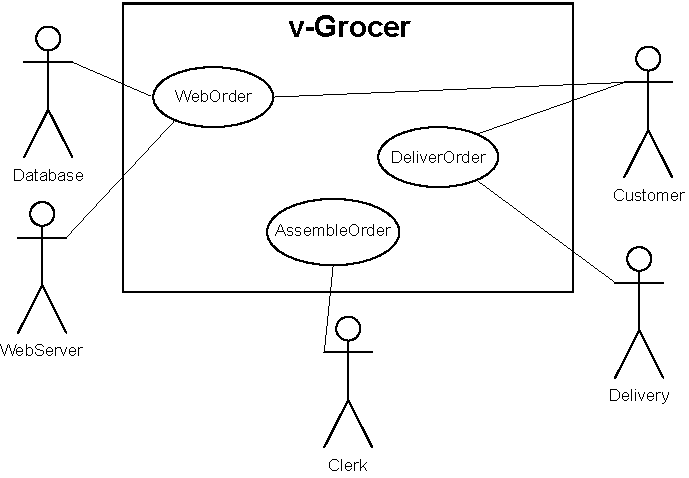
\includegraphics{media/image10.wmf}, that reflect the technical merit of
each of the \emph{j\textsuperscript{th}} design options relative to
\emph{i\textsuperscript{th}} criterion. The total score,
\emph{S\textsubscript{j}}, for each design option is computed as a
weighted summation of the design ratings and weighting factors.

\textbf{Table 4.4} A decision matrix for the Analytical Hierarchy
Process.

\begin{longtable}[]{@{}
  >{\raggedright\arraybackslash}p{(\columnwidth - 10\tabcolsep) * \real{0.1377}}
  >{\raggedright\arraybackslash}p{(\columnwidth - 10\tabcolsep) * \real{0.0975}}
  >{\raggedright\arraybackslash}p{(\columnwidth - 10\tabcolsep) * \real{0.2085}}
  >{\raggedright\arraybackslash}p{(\columnwidth - 10\tabcolsep) * \real{0.2111}}
  >{\raggedright\arraybackslash}p{(\columnwidth - 10\tabcolsep) * \real{0.1341}}
  >{\raggedright\arraybackslash}p{(\columnwidth - 10\tabcolsep) * \real{0.2111}}@{}}
\toprule\noalign{}
\multicolumn{2}{@{}>{\raggedright\arraybackslash}p{(\columnwidth - 10\tabcolsep) * \real{0.2352} + 2\tabcolsep}}{%
\begin{minipage}[b]{\linewidth}\raggedright
\end{minipage}} & \begin{minipage}[b]{\linewidth}\raggedright
\textbf{Design Option 1}
\end{minipage} & \begin{minipage}[b]{\linewidth}\raggedright
\textbf{Design Option 2}
\end{minipage} & \begin{minipage}[b]{\linewidth}\raggedright
\end{minipage} & \begin{minipage}[b]{\linewidth}\raggedright
\textbf{Design Option n}
\end{minipage} \\
\midrule\noalign{}
\endhead
\bottomrule\noalign{}
\endlastfoot
\textbf{Criteria 1} & 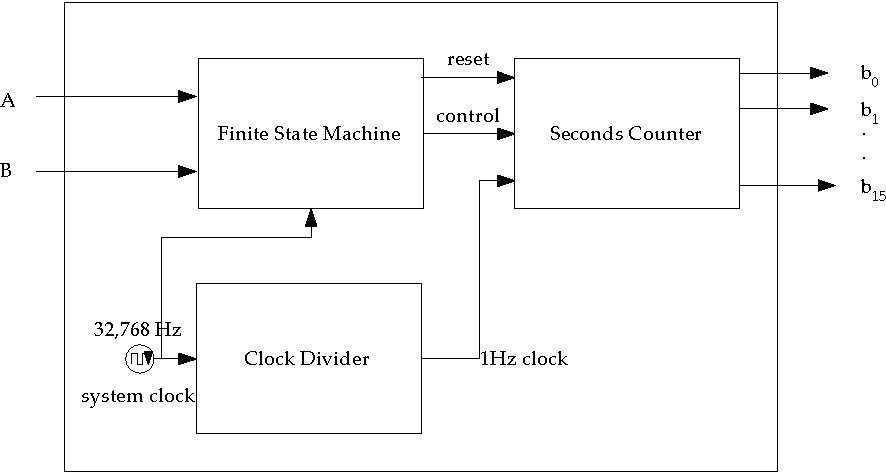
\includegraphics{media/image11.wmf} &
\emph{α\textsubscript{11}} & \emph{α\textsubscript{12}} &

\includegraphics{media/image12.wmf} & \emph{α\textsubscript{1n}} \\
\textbf{Criteria 2} & 
\includegraphics{media/image13.wmf} &
\emph{α\textsubscript{21}} & \emph{α\textsubscript{22}} &

\includegraphics{media/image14.wmf} & \emph{α\textsubscript{2n}} \\
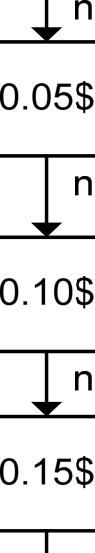
\includegraphics{media/image15.wmf} &
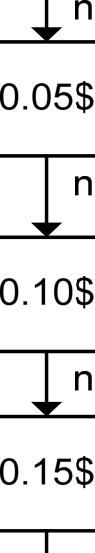
\includegraphics{media/image15.wmf} &
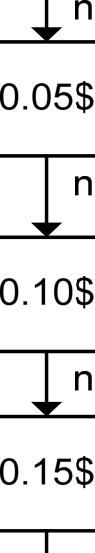
\includegraphics{media/image15.wmf} &
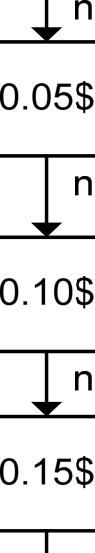
\includegraphics{media/image15.wmf} &

\includegraphics{media/image14.wmf} &
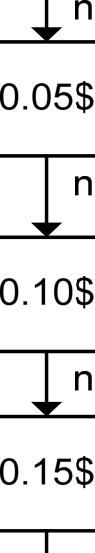
\includegraphics{media/image15.wmf} \\
\textbf{Criteria \emph{m}} & 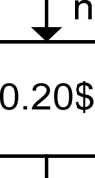
\includegraphics{media/image16.wmf} &
\emph{α\textsubscript{m1}} & \emph{α\textsubscript{m2}} &

\includegraphics{media/image14.wmf} & \emph{α\textsubscript{mn}} \\
\multicolumn{2}{@{}>{\raggedright\arraybackslash}p{(\columnwidth - 10\tabcolsep) * \real{0.2352} + 2\tabcolsep}}{%
\textbf{Score}} & 
\includegraphics{media/image17.wmf} &
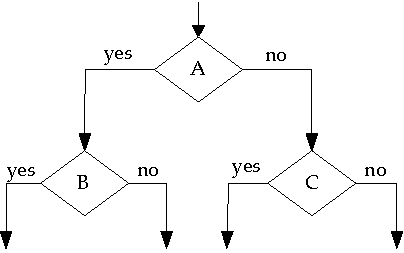
\includegraphics{media/image18.wmf} &

\includegraphics{media/image14.wmf} &

\includegraphics{media/image19.wmf} \\
\end{longtable}

The application of AHP is demonstrated for the design of an electronic
circuit for measuring temperature, by producing a voltage signal that is
directly proportional to temperature.

\subsubsection*{Step 1: Determine the Selection
Criteria}\label{step-1-determine-the-selection-criteria}
\addcontentsline{toc}{subsubsection}{Step 1: Determine the Selection
Criteria}

Assume that the criteria for comparing the concepts are high accuracy,
low cost, small size, and availability of parts for manufacture.

\subsubsection*{Step 2: Determine the Criteria
Weightings}\label{step-2-determine-the-criteria-weightings}
\addcontentsline{toc}{subsubsection}{Step 2: Determine the Criteria
Weightings}

\begin{itemize}
\item
  Assume that the criteria were ranked using pairwise comparison and
  weights computed (see Appendix B) as shown in Table 4.5.
\end{itemize}

\textbf{Table 4.5} Pairwise comparison matrix.

\begin{longtable}[]{@{}
  >{\raggedright\arraybackslash}p{(\columnwidth - 10\tabcolsep) * \real{0.2370}}
  >{\raggedright\arraybackslash}p{(\columnwidth - 10\tabcolsep) * \real{0.1473}}
  >{\raggedright\arraybackslash}p{(\columnwidth - 10\tabcolsep) * \real{0.1399}}
  >{\raggedright\arraybackslash}p{(\columnwidth - 10\tabcolsep) * \real{0.1354}}
  >{\raggedright\arraybackslash}p{(\columnwidth - 10\tabcolsep) * \real{0.1640}}
  >{\raggedright\arraybackslash}p{(\columnwidth - 10\tabcolsep) * \real{0.1764}}@{}}
\toprule\noalign{}
\begin{minipage}[b]{\linewidth}\raggedright
\end{minipage} & \begin{minipage}[b]{\linewidth}\raggedright
\textbf{Accuracy}
\end{minipage} & \begin{minipage}[b]{\linewidth}\raggedright
\textbf{Cost}
\end{minipage} & \begin{minipage}[b]{\linewidth}\raggedright
\textbf{Size}
\end{minipage} & \begin{minipage}[b]{\linewidth}\raggedright
\textbf{Availability}
\end{minipage} & \begin{minipage}[b]{\linewidth}\raggedright
\textbf{Weights}
\end{minipage} \\
\midrule\noalign{}
\endhead
\bottomrule\noalign{}
\endlastfoot
\textbf{Accuracy} & 1 & 5 & 3 & ¼ & 0.42 \\
\textbf{Cost} & 1/5 & 1 & \begin{minipage}[t]{\linewidth}\raggedright
\begin{quote}
2
\end{quote}
\end{minipage} & ¼ & 0.12 \\
\textbf{Size} & 1/3 & ½ & 1 & 1 & 0.12 \\
\textbf{Availability} & \begin{minipage}[t]{\linewidth}\raggedright
\begin{quote}
4
\end{quote}
\end{minipage} & \begin{minipage}[t]{\linewidth}\raggedright
\begin{quote}
4
\end{quote}
\end{minipage} & \begin{minipage}[t]{\linewidth}\raggedright
\begin{quote}
1
\end{quote}
\end{minipage} & 1 & 0.34 \\
\end{longtable}

\subsubsection*{Step 3: Identify and Rate Alternatives Relative to the
Criteria}\label{step-3-identify-and-rate-alternatives-relative-to-the-criteria}
\addcontentsline{toc}{subsubsection}{Step 3: Identify and Rate
Alternatives Relative to the Criteria}

Three candidate solutions are shown in Figure 4.6. Each acts as a
constant current source that drives a temperature measurement device
(RTD). The resistance of an RTD varies with temperature, and when driven
by a constant cur­rent, \emph{I}, produces a voltage,
\emph{V\textsubscript{T}}, that varies proportionally with temperature.
Each circuit supplies a constant current of I=1mA.

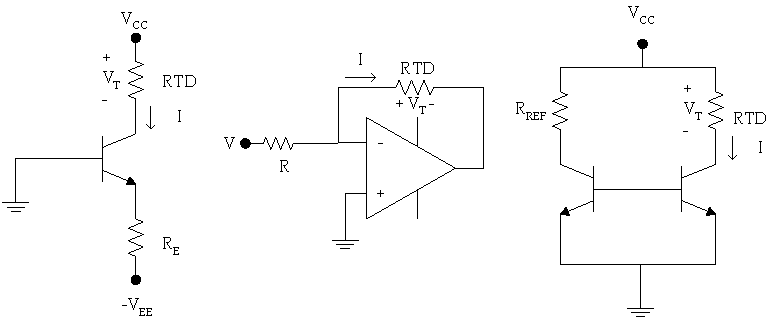
\includegraphics[width=5.5in,height=2.32292in]{media/image20.emf}

\textbf{1: Single Transistor 2: Inverting Op Amp 3: Current Mirror}

\textbf{Figure 4.6} Candidate solutions for temperature measurement.

The accuracy of each design was evaluated by a sensitivity analysis
using a SPICE cir­cuit simulation package assuming 10\% resistors. The
deviation of the output volt­age (maximum deviation from nominal) for the
three designs is 9.2\%, 1.3\%, and 1.9\% respectively. Since the
objective is to minimize the deviation, the following rating metric is
used


\includegraphics{media/image21.wmf}. (1)

This produces the following normalize design ratings for accuracy:

\includegraphics{media/image22.wmf} \emph{=} 0.08,
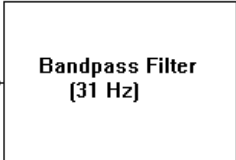
\includegraphics{media/image23.wmf} \emph{=} 0.55, and

\includegraphics{media/image24.wmf} \emph{=} 0.37.

The parts costs are the following: resistors = \$0.05, bipolar junction
transistors (BJTs) = \$0.15, op amps = \$0.35, and RTDs = \$0.25. Using
a measure for cost similar to (1) gives following normalized cost
ratings for the three options
respec­tively:
\includegraphics{media/image25.wmf} \emph{=} 0.41,

\includegraphics{media/image26.wmf} \emph{=} 0.28, and

\includegraphics{media/image27.wmf} \emph{=} 0.31.

Assume that to manufacture each circuit on a printed circuit board
requires the following dimen­sions: design 1 = 1 in\textsuperscript{2},
design 2 = 1.56 in\textsuperscript{2}, and design 3 = 2.25
in\textsuperscript{2}. The objective is to minimize size, and againusing
a measure analogous to (1) for the required space to manufacture each
produces the following normalized decision ratings:

\includegraphics{media/image28.wmf} = 0.48,

\includegraphics{media/image29.wmf} = 0.31, and

\includegraphics{media/image30.wmf} = 0.21.

Assume that the parts have an in-stock availability of 95\%, 70\%, 90\%,
and 80\% of the time for the resistors, BJTs, RTDs, and op amps
respectively. A measure for the overall availability of parts to
manufacture each design is re­quired. One way to measure this is to
compute the probability that a design will be able to be manufactured
based upon the past history of part availability. This is found by
multiplying the availability of all individual components needed for the
design:

\emph{P}(design 1 can be produced) \emph{=} (0.95)(0.90)(0.70) = 0.60

\emph{P}(design 2 can be produced) \emph{=} (0.95)(0.90)(0.80) = 0.68

\emph{P}(design 3 can be produced) \emph{=} (0.95)(0.90) (0.70)(0.70) =
0.42

This produces the following normalized decision ratings for
availability: 
\includegraphics{media/image31.wmf} = 0.35,

\includegraphics{media/image32.wmf} = 0.40, and

\includegraphics{media/image33.wmf} = 0.25.

\subsubsection*{Step 4: Compute Scores for the
Alternatives}\label{step-4-compute-scores-for-the-alternatives}
\addcontentsline{toc}{subsubsection}{Step 4: Compute Scores for the
Alternatives}

The decision matrix is built and the overall weighted scores for the
alternatives are computed as shown in Table 4.6.

\textbf{Table 4.6} The decision matrix.

\begin{longtable}[]{@{}
  >{\raggedright\arraybackslash}p{(\columnwidth - 8\tabcolsep) * \real{0.1823}}
  >{\raggedright\arraybackslash}p{(\columnwidth - 8\tabcolsep) * \real{0.1028}}
  >{\raggedright\arraybackslash}p{(\columnwidth - 8\tabcolsep) * \real{0.2373}}
  >{\raggedright\arraybackslash}p{(\columnwidth - 8\tabcolsep) * \real{0.2400}}
  >{\raggedright\arraybackslash}p{(\columnwidth - 8\tabcolsep) * \real{0.2376}}@{}}
\toprule\noalign{}
\multicolumn{2}{@{}>{\raggedright\arraybackslash}p{(\columnwidth - 8\tabcolsep) * \real{0.2851} + 2\tabcolsep}}{%
\begin{minipage}[b]{\linewidth}\raggedright
\end{minipage}} & \begin{minipage}[b]{\linewidth}\raggedright
\textbf{Single BJT}
\end{minipage} & \begin{minipage}[b]{\linewidth}\raggedright
\textbf{Op Amp}
\end{minipage} & \begin{minipage}[b]{\linewidth}\raggedright
\textbf{Current Mirror}
\end{minipage} \\
\midrule\noalign{}
\endhead
\bottomrule\noalign{}
\endlastfoot
\textbf{Accuracy} & 0.42 & 0.08 & 0.55 & 0.37 \\
\textbf{Cost} & 0.12 & 0.41 & 0.28 & 0.31 \\
\textbf{Size} & 0.12 & 0.48 & 0.31 & 0.21 \\
\textbf{Availability} & 0.34 & 0.35 & 0.40 & 0.25 \\
\multicolumn{2}{@{}>{\raggedright\arraybackslash}p{(\columnwidth - 8\tabcolsep) * \real{0.2851} + 2\tabcolsep}}{%
\emph{\textbf{Score}}} & 0.26 & 0.44 & 0.30 \\
\end{longtable}

\subsubsection*{Step 5: Review the
Decision}\label{step-5-review-the-decision}
\addcontentsline{toc}{subsubsection}{Step 5: Review the Decision}

Remember that this is a semi-quantitative method. The final ranking
indicates that design options 1 and 3 are quite similar, while both are
inferior to option 2.

\subsubsection{Pugh Concept Selection}\label{pugh-concept-selection}

Pugh Concept Selection is a method of comparing concepts against
criteria, similar to what we saw with a decision matrix. It is different
in that it has a simpler scoring method and it is an iterative process.
The steps of Pugh Concept Selection are:

\begin{enumerate}
\def\labelenumi{\arabic{enumi}.}
\item
  Select the comparison criteria, usually the engineering or marketing
  requirements.
\item
  Determine weights for the criterion.
\item
  Determine the concepts.
\item
  Select a baseline concept that is initially believed to be the best.
\item
  Compare all other concepts to the baseline, using the following
  scoring method: +1 better than, 0 equal to, -1 worse than.
\item
  Compute a weighted score for each concept, not including the baseline.
\item
  Examine each concept to determine if it should be retained, updated,
  or dropped. Synthesize the best elements of others into other concepts
  wherever possible.
\item
  Update the table and iterate until a superior concept emerges.
\end{enumerate}

An example of a Pugh Concept Selection matrix is shown in Table 4.7.

\textbf{Table 4.7} Pugh Concept Selection matrix.

\begin{longtable}[]{@{}
  >{\raggedright\arraybackslash}p{(\columnwidth - 10\tabcolsep) * \real{0.1630}}
  >{\raggedright\arraybackslash}p{(\columnwidth - 10\tabcolsep) * \real{0.1155}}
  >{\raggedright\arraybackslash}p{(\columnwidth - 10\tabcolsep) * \real{0.1889}}
  >{\raggedright\arraybackslash}p{(\columnwidth - 10\tabcolsep) * \real{0.1848}}
  >{\raggedright\arraybackslash}p{(\columnwidth - 10\tabcolsep) * \real{0.1739}}
  >{\raggedright\arraybackslash}p{(\columnwidth - 10\tabcolsep) * \real{0.1739}}@{}}
\toprule\noalign{}
\multicolumn{2}{@{}>{\raggedright\arraybackslash}p{(\columnwidth - 10\tabcolsep) * \real{0.2785} + 2\tabcolsep}}{%
\begin{minipage}[b]{\linewidth}\raggedright
\end{minipage}} & \begin{minipage}[b]{\linewidth}\raggedright
\textbf{Option 1}

\textbf{(Reference)}
\end{minipage} & \begin{minipage}[b]{\linewidth}\raggedright
\textbf{Option 2}
\end{minipage} & \begin{minipage}[b]{\linewidth}\raggedright
\textbf{Option 3}
\end{minipage} & \begin{minipage}[b]{\linewidth}\raggedright
\textbf{Option 4}
\end{minipage} \\
\midrule\noalign{}
\endhead
\bottomrule\noalign{}
\endlastfoot
\textbf{Criteria 1} & 4 & - & 0 & 0 & +1 \\
\textbf{Criteria 2} & 5 & - & +1 & -1 & 0 \\
\textbf{Criteria 3} & 2 & - & -1 & 0 & +1 \\
\textbf{Criteria 4} & 1 & - & +1 & +1 & -1 \\
\multicolumn{2}{@{}>{\raggedright\arraybackslash}p{(\columnwidth - 10\tabcolsep) * \real{0.2785} + 2\tabcolsep}}{%
\textbf{Score}} & - & 4 & -4 & 5 \\
\multicolumn{2}{@{}>{\raggedright\arraybackslash}p{(\columnwidth - 10\tabcolsep) * \real{0.2785} + 2\tabcolsep}}{%
\textbf{Continue?}} & Combine & Yes & No & Combine \\
\end{longtable}

\subsection{Project Application: Concept Generation and
Evaluation}\label{project-application-concept-generation-and-evaluation}

The following advice is provided for teams in the concept generation and
evaluation phase:

\begin{itemize}
\item
  Set aside time specifically for concept generation and evaluation and
  take it as a challenge to identify as many concepts as possible.
\item
  Search externally, including literature reviews and patent searches.
\item
  Search internally using brainstorming, brainwriting, or the Nominal
  Group Technique. Effective teams generate many concepts in a
  brainstorming session.
\item
  Examine solutions for the entire design, for sub-functions of the
  design, and for individual components (such as integrated circuit
  selection). The tech­niques in this chapter can be combined with design
  methods presented in Chapters 5 and 6.
\item
  Utilize SCAMPER, concept tables, and concepts fans as tools to
  facilitate and document concept generation.
\item
  Critically and objectively evaluate concepts against common criteria.
\item
  Clearly identify the concept(s) selected and the rationale for
  selection.
\end{itemize}

\subsection{Summary and Further
Reading}\label{summary-and-further-reading}

In the design process, it is important to creatively generate different
concepts for a solution to a problem. This is followed by an evaluation
of concepts to determine which are the most promising. This chapter
identified barriers to creativity and provided strategies for enhancing
creative ability. The concepts of vertical and lateral thinking were
introduced, and their im­pact on the design process was explored. Methods
of concept generation, including brainstorming, concept tables, and
concepts fans were presented. Finally, methods for critically evaluating
concepts (strength/weakness analysis, Analytical Hierarchy Process, and
Pugh Concept selection) were presented.

There are many references that examine creativity and concept
generation. Adams {[}Ada01{]} is a good reference for creativity and
problem-solving with a technical bent. Alex Os­born was an advocate of
creativity and developed two readable works that address the creative
process, the need for creativity, and strategies for enhancing it
{[}Osb48, Osb63{]}. Ed­ward DeBono is another well-known authority in the
field and has produced many works on lateral thinking and creativity
{[}Deb67, Deb70{]}. Paul Sloane has published numerous books with
lateral thinking puzzles {[}Slo91, Slo93, Slo94{]}. TRIZ {[}Alt99{]} is
a more advanced and complex approach to concept generation, that centers
around resolving tradeoffs in a problem. It is fairly complex and may be
considered by more advanced teams.

\subsection{Problems}\label{problems}

\begin{enumerate}
\def\labelenumi{\arabic{enumi}.}
\item
  Consider the nine dot puzzle shown in Figure 4.1 (b). Draw
  \textbf{three} connected straight lines that pass through all nine
  dots.
\end{enumerate}

\begin{enumerate}
\def\labelenumi{\arabic{enumi}.}
\item
  Consider the six sticks shown below. Rearrange the sticks to produce
  four equilat­eral triangles (the sticks cannot be broken).
\item
  Consider the fish shown below made of eight sticks and a coin for the
  eye. The objective is to make the fish face the other direction by
  moving only the coin and three sticks.
\end{enumerate}


\includegraphics[width=2in,height=1.35417in]{media/image34.emf}

\begin{enumerate}
\def\labelenumi{\arabic{enumi}.}
\setcounter{enumi}{2}
\item
  For each of the following lateral thinking puzzles, develop a
  plausible solution (from Paul Sloane's \ul{Lateral Thinking Puzzles}
  {[}http://dspace.dial.pipex.com/sloane{]}):
\end{enumerate}

\begin{enumerate}
\def\labelenumi{\alph{enumi}.}
\item
  A man walks into a bar and asks the barman for a glass of water. The
  barman pulls out a gun and points it at the man. The man says
  \textquotesingle Thank you\textquotesingle{} and walks out.
\item
  A woman had two sons who were born on the same hour of the same day of
  the same year. But they were not twins. How could this be so?
\item
  Why is it better to have round manhole covers than square ones?
\item
  A man went to a party and drank some of the punch. He then left early.
  Everyone else at the party who drank the punch subsequently died of
  poisoning. Why did the man not die?
\end{enumerate}

\begin{enumerate}
\def\labelenumi{\arabic{enumi}.}
\setcounter{enumi}{4}
\item
  Legislation was passed to allow handguns in the cockpits of passenger
  airliners to prevent hijacking. Brainstorm to develop concepts that
  prevent anyone other than the pilot from using the handgun.
\item
  Imagine if scientists and engineers were able to develop a technology
  that would allow people to be transported from any place on earth to
  another instantaneously. Brainstorm to determine the potential impact
  this would have on society.
\item
  Student advising at many colleges and universities is seen as an area
  that can be im­proved. Brainstorm to develop ideas as to how student
  advising could be improved at your college or university.
\item
  In your own words, describe what a concept table and a concept fan
  are.
\item
  Consider the problem solved in Section 4.3.2. For this example assume
  that:
\end{enumerate}

\begin{itemize}
\item
  The following is the result of the paired comparison.
\end{itemize}

\begin{longtable}[]{@{}
  >{\raggedright\arraybackslash}p{(\columnwidth - 8\tabcolsep) * \real{0.2212}}
  >{\raggedright\arraybackslash}p{(\columnwidth - 8\tabcolsep) * \real{0.1974}}
  >{\raggedright\arraybackslash}p{(\columnwidth - 8\tabcolsep) * \real{0.1810}}
  >{\raggedright\arraybackslash}p{(\columnwidth - 8\tabcolsep) * \real{0.1794}}
  >{\raggedright\arraybackslash}p{(\columnwidth - 8\tabcolsep) * \real{0.2211}}@{}}
\toprule\noalign{}
\begin{minipage}[b]{\linewidth}\raggedright
\end{minipage} & \begin{minipage}[b]{\linewidth}\raggedright
Accuracy
\end{minipage} & \begin{minipage}[b]{\linewidth}\raggedright
Cost
\end{minipage} & \begin{minipage}[b]{\linewidth}\raggedright
Size
\end{minipage} & \begin{minipage}[b]{\linewidth}\raggedright
Availability
\end{minipage} \\
\midrule\noalign{}
\endhead
\bottomrule\noalign{}
\endlastfoot
Accuracy & 1 & 1/3 & 2 & ½ \\
Cost & 3 & 1 & 5 & 1 \\
Size & 1/2 & 1/5 & 1 & 2 \\
Availability & 2 & 1 & ½ & 1 \\
\end{longtable}

\begin{itemize}
\item
  The parts costs are the following: resistors = \$0.05, bipolar
  transistors (BJTs) = \$0.10, op amps = \$0.35, and RTDs = \$0.25.
\item
  The parts have an in-stock availability of 99\%, 90\%, 85\%, and 70\%
  of the time for the re­sistors, BJTs, RTDs, and op amps respectively.
\item
  Everything else is the same as presented in Section 4.3.2.
\end{itemize}

\begin{quote}
Compute the rankings of the design options using a weighted decision
matrix of the type shown in Table 4.5.
\end{quote}

\begin{enumerate}
\def\labelenumi{\arabic{enumi}.}
\item
  \textbf{Project Application.} Utilize the methods in this chapter to
  generate con­cepts for your particular design problem. Critically
  evaluate the concepts generated using one or more of the techniques
  presented in the chapter that is appropriate for the problem. Section
  4.4 pro­vides guidance on how to conduct this process and document the
  results.
\end{enumerate}

\textbf{Concept Generation}
